\documentclass[1p]{elsarticle_modified}
%\bibliographystyle{elsarticle-num}

%\usepackage[colorlinks]{hyperref}
%\usepackage{abbrmath_seonhwa} %\Abb, \Ascr, \Acal ,\Abf, \Afrak
\usepackage{amsfonts}
\usepackage{amssymb}
\usepackage{amsmath}
\usepackage{amsthm}
\usepackage{scalefnt}
\usepackage{amsbsy}
\usepackage{kotex}
\usepackage{caption}
\usepackage{subfig}
\usepackage{color}
\usepackage{graphicx}
\usepackage{xcolor} %% white, black, red, green, blue, cyan, magenta, yellow
\usepackage{float}
\usepackage{setspace}
\usepackage{hyperref}

\usepackage{tikz}
\usetikzlibrary{arrows}

\usepackage{multirow}
\usepackage{array} % fixed length table
\usepackage{hhline}

%%%%%%%%%%%%%%%%%%%%%
\makeatletter
\renewcommand*\env@matrix[1][\arraystretch]{%
	\edef\arraystretch{#1}%
	\hskip -\arraycolsep
	\let\@ifnextchar\new@ifnextchar
	\array{*\c@MaxMatrixCols c}}
\makeatother %https://tex.stackexchange.com/questions/14071/how-can-i-increase-the-line-spacing-in-a-matrix
%%%%%%%%%%%%%%%

\usepackage[normalem]{ulem}

\newcommand{\msout}[1]{\ifmmode\text{\sout{\ensuremath{#1}}}\else\sout{#1}\fi}
%SOURCE: \msout is \stkout macro in https://tex.stackexchange.com/questions/20609/strikeout-in-math-mode

\newcommand{\cancel}[1]{
	\ifmmode
	{\color{red}\msout{#1}}
	\else
	{\color{red}\sout{#1}}
	\fi
}

\newcommand{\add}[1]{
	{\color{blue}\uwave{#1}}
}

\newcommand{\replace}[2]{
	\ifmmode
	{\color{red}\msout{#1}}{\color{blue}\uwave{#2}}
	\else
	{\color{red}\sout{#1}}{\color{blue}\uwave{#2}}
	\fi
}

\newcommand{\Sol}{\mathcal{S}} %segment
\newcommand{\D}{D} %diagram
\newcommand{\A}{\mathcal{A}} %arc


%%%%%%%%%%%%%%%%%%%%%%%%%%%%%5 test

\def\sl{\operatorname{\textup{SL}}(2,\Cbb)}
\def\psl{\operatorname{\textup{PSL}}(2,\Cbb)}
\def\quan{\mkern 1mu \triangleright \mkern 1mu}

\theoremstyle{definition}
\newtheorem{thm}{Theorem}[section]
\newtheorem{prop}[thm]{Proposition}
\newtheorem{lem}[thm]{Lemma}
\newtheorem{ques}[thm]{Question}
\newtheorem{cor}[thm]{Corollary}
\newtheorem{defn}[thm]{Definition}
\newtheorem{exam}[thm]{Example}
\newtheorem{rmk}[thm]{Remark}
\newtheorem{alg}[thm]{Algorithm}

\newcommand{\I}{\sqrt{-1}}
\begin{document}

%\begin{frontmatter}
%
%\title{Boundary parabolic representations of knots up to 8 crossings}
%
%%% Group authors per affiliation:
%\author{Yunhi Cho} 
%\address{Department of Mathematics, University of Seoul, Seoul, Korea}
%\ead{yhcho@uos.ac.kr}
%
%
%\author{Seonhwa Kim} %\fnref{s_kim}}
%\address{Center for Geometry and Physics, Institute for Basic Science, Pohang, 37673, Korea}
%\ead{ryeona17@ibs.re.kr}
%
%\author{Hyuk Kim}
%\address{Department of Mathematical Sciences, Seoul National University, Seoul 08826, Korea}
%\ead{hyukkim@snu.ac.kr}
%
%\author{Seokbeom Yoon}
%\address{Department of Mathematical Sciences, Seoul National University, Seoul, 08826,  Korea}
%\ead{sbyoon15@snu.ac.kr}
%
%\begin{abstract}
%We find all boundary parabolic representation of knots up to 8 crossings.
%
%\end{abstract}
%\begin{keyword}
%    \MSC[2010] 57M25 
%\end{keyword}
%
%\end{frontmatter}

%\linenumbers
%\tableofcontents
%
\newcommand\colored[1]{\textcolor{white}{\rule[-0.35ex]{0.8em}{1.4ex}}\kern-0.8em\color{red} #1}%
%\newcommand\colored[1]{\textcolor{white}{ #1}\kern-2.17ex	\textcolor{white}{ #1}\kern-1.81ex	\textcolor{white}{ #1}\kern-2.15ex\color{red}#1	}

{\Large $\underline{10_{156}~(K10n_{32})}$}

\setlength{\tabcolsep}{10pt}
\renewcommand{\arraystretch}{1.6}
\vspace{1cm}\begin{tabular}{m{100pt}>{\centering\arraybackslash}m{274pt}}
\multirow{5}{120pt}{
	\centering
	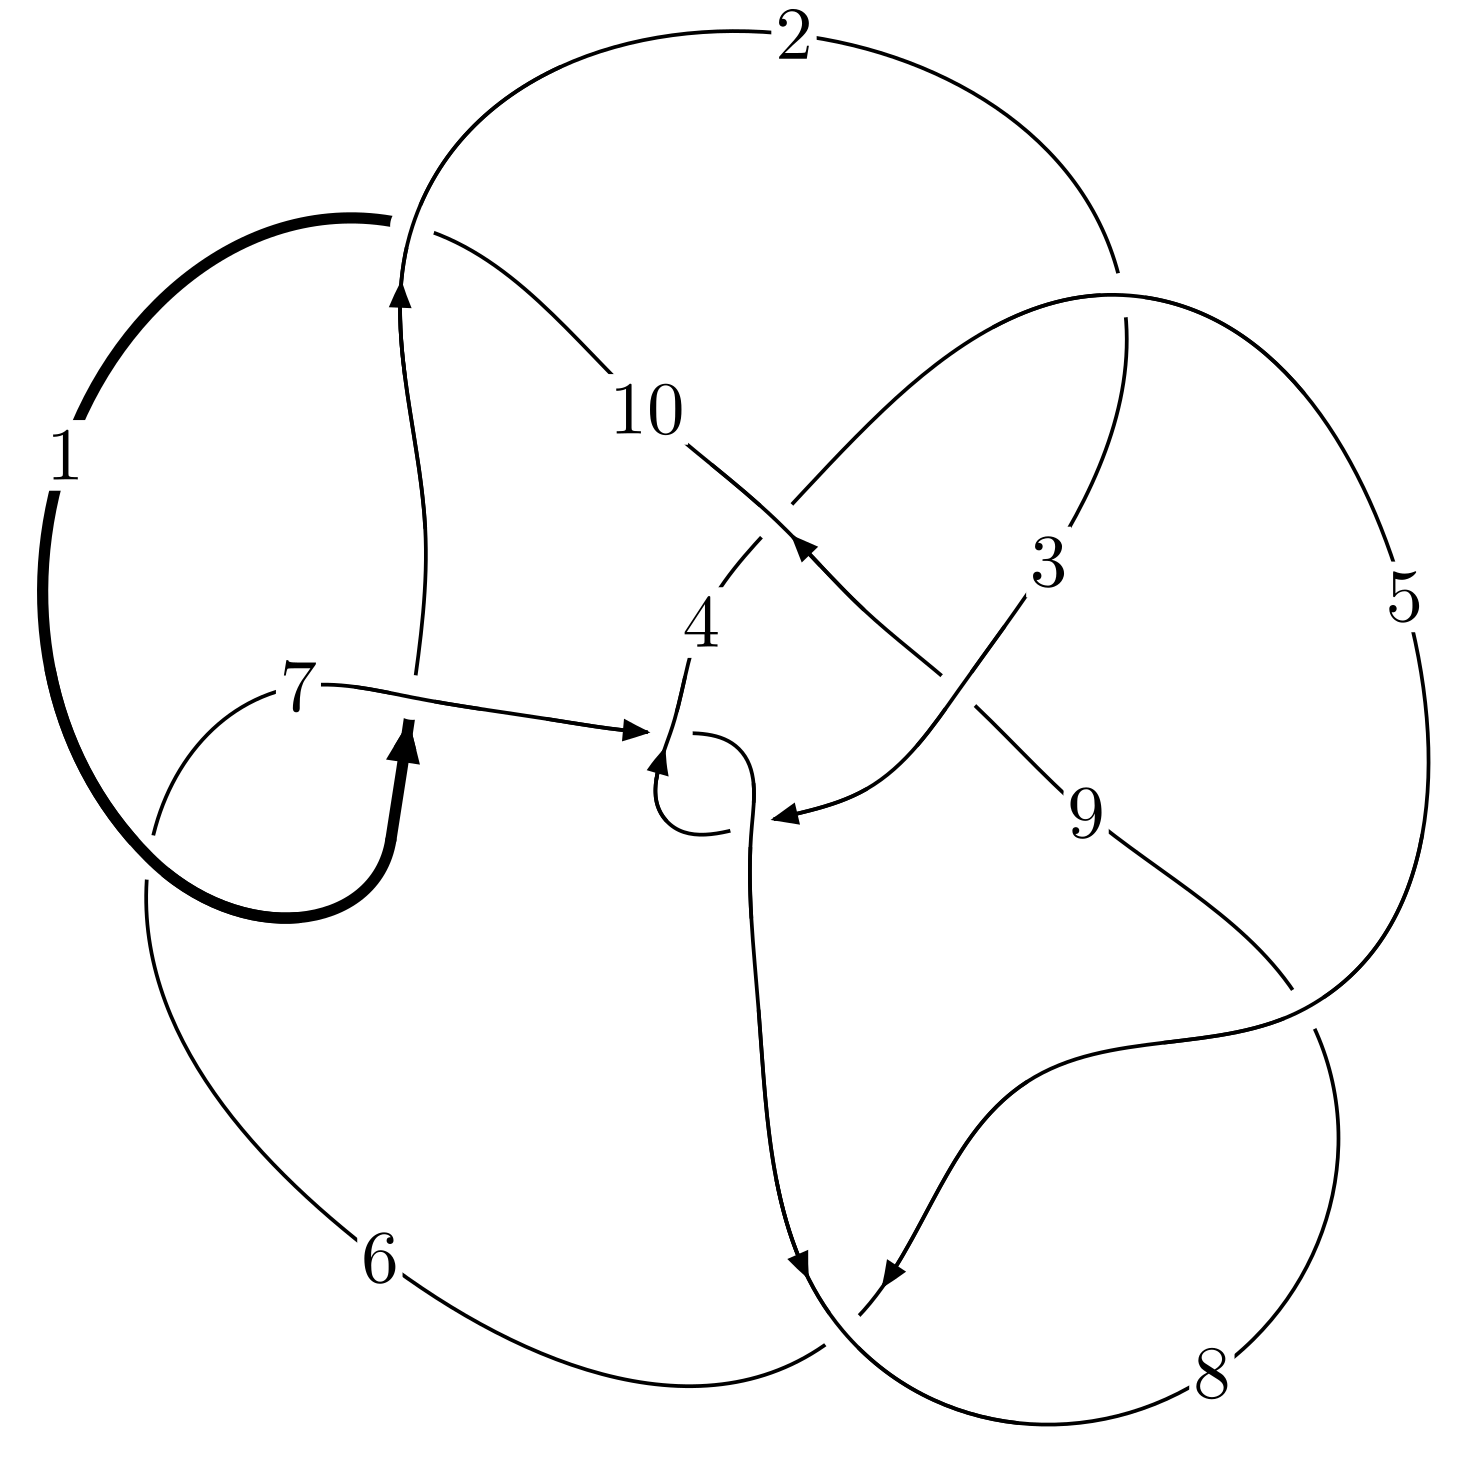
\includegraphics[width=112pt]{../../../GIT/diagram.site/Diagrams/png/240_10_156.png}\\
\ \ \ A knot diagram\footnotemark}&
\allowdisplaybreaks
\textbf{Linearized knot diagam} \\
\cline{2-2}
 &
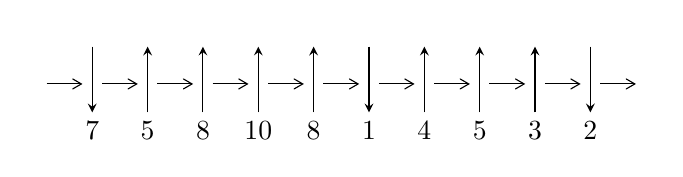
\begin{tikzpicture}[x=20pt, y=17pt]
	% nodes
	\node (C0) at (0, 0) {};
	\node (C1) at (1, 0) {};
	\node (C1U) at (1, +1) {};
	\node (C1D) at (1, -1) {7};

	\node (C2) at (2, 0) {};
	\node (C2U) at (2, +1) {};
	\node (C2D) at (2, -1) {5};

	\node (C3) at (3, 0) {};
	\node (C3U) at (3, +1) {};
	\node (C3D) at (3, -1) {8};

	\node (C4) at (4, 0) {};
	\node (C4U) at (4, +1) {};
	\node (C4D) at (4, -1) {10};

	\node (C5) at (5, 0) {};
	\node (C5U) at (5, +1) {};
	\node (C5D) at (5, -1) {8};

	\node (C6) at (6, 0) {};
	\node (C6U) at (6, +1) {};
	\node (C6D) at (6, -1) {1};

	\node (C7) at (7, 0) {};
	\node (C7U) at (7, +1) {};
	\node (C7D) at (7, -1) {4};

	\node (C8) at (8, 0) {};
	\node (C8U) at (8, +1) {};
	\node (C8D) at (8, -1) {5};

	\node (C9) at (9, 0) {};
	\node (C9U) at (9, +1) {};
	\node (C9D) at (9, -1) {3};

	\node (C10) at (10, 0) {};
	\node (C10U) at (10, +1) {};
	\node (C10D) at (10, -1) {2};
	\node (C11) at (11, 0) {};

	% arrows
	\draw[->,>={angle 60}]
	(C0) edge (C1) (C1) edge (C2) (C2) edge (C3) (C3) edge (C4) (C4) edge (C5) (C5) edge (C6) (C6) edge (C7) (C7) edge (C8) (C8) edge (C9) (C9) edge (C10) (C10) edge (C11) ;	\draw[->,>=stealth]
	(C1U) edge (C1D) (C2D) edge (C2U) (C3D) edge (C3U) (C4D) edge (C4U) (C5D) edge (C5U) (C6U) edge (C6D) (C7D) edge (C7U) (C8D) edge (C8U) (C9D) edge (C9U) (C10U) edge (C10D) ;
	\end{tikzpicture} \\
\hhline{~~} \\& 
\textbf{Solving Sequence} \\ \cline{2-2} 
 &
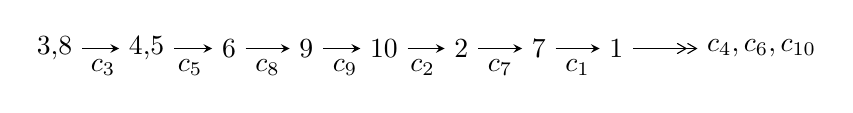
\begin{tikzpicture}[x=28pt, y=7pt]
	% node
	\node (A0) at (-1/8, 0) {3,8};
	\node (A1) at (17/16, 0) {4,5};
	\node (A2) at (17/8, 0) {6};
	\node (A3) at (25/8, 0) {9};
	\node (A4) at (33/8, 0) {10};
	\node (A5) at (41/8, 0) {2};
	\node (A6) at (49/8, 0) {7};
	\node (A7) at (57/8, 0) {1};
	\node (C1) at (1/2, -1) {$c_{3}$};
	\node (C2) at (13/8, -1) {$c_{5}$};
	\node (C3) at (21/8, -1) {$c_{8}$};
	\node (C4) at (29/8, -1) {$c_{9}$};
	\node (C5) at (37/8, -1) {$c_{2}$};
	\node (C6) at (45/8, -1) {$c_{7}$};
	\node (C7) at (53/8, -1) {$c_{1}$};
	\node (A8) at (9, 0) {$c_{4},c_{6},c_{10}$};

	% edge
	\draw[->,>=stealth]	
	(A0) edge (A1) (A1) edge (A2) (A2) edge (A3) (A3) edge (A4) (A4) edge (A5) (A5) edge (A6) (A6) edge (A7) ;
	\draw[->>,>={angle 60}]	
	(A7) edge (A8);
\end{tikzpicture} \\ 

\end{tabular} \\

\footnotetext{
The image of knot diagram is generated by the software ``\textbf{Draw programme}" developed by Andrew Bartholomew(\url{http://www.layer8.co.uk/maths/draw/index.htm\#Running-draw}), where we modified some parts for our purpose(\url{https://github.com/CATsTAILs/LinksPainter}).
}\phantom \\ \newline 
\centering \textbf{Ideals for irreducible components\footnotemark of $X_{\text{par}}$} 
 
\begin{align*}
I^u_{1}&=\langle 
-4 u^9-2 u^8- u^7+9 u^6-29 u^5- u^4+13 u^3+51 u^2+27 b-19 u+8,\\
\phantom{I^u_{1}}&\phantom{= \langle  }-11 u^9+8 u^8+4 u^7-9 u^6-46 u^5+31 u^4+29 u^3+12 u^2+27 a-32 u-5,\;u^{10}+u^7+5 u^6- u^3+u^2- u+1\rangle \\
I^u_{2}&=\langle 
u^2+b+1,\;u^3+a+2 u+1,\;u^5+2 u^3+u^2+1\rangle \\
I^u_{3}&=\langle 
-3646 u^{11}+4692 u^{10}+\cdots+3395 b+12871,\;24747 u^{11}-25539 u^{10}+\cdots+16975 a-130862,\\
\phantom{I^u_{3}}&\phantom{= \langle  }u^{12}- u^{11}+2 u^{10}-3 u^9+6 u^8-3 u^7+9 u^6-5 u^5-2 u^4-8 u^2-6 u-1\rangle \\
\\
\end{align*}
\raggedright * 3 irreducible components of $\dim_{\mathbb{C}}=0$, with total 27 representations.\\
\footnotetext{All coefficients of polynomials are rational numbers. But the coefficients are sometimes approximated in decimal forms when there is not enough margin.}
\newpage
\renewcommand{\arraystretch}{1}
\centering \section*{I. $I^u_{1}= \langle -4 u^9-2 u^8+\cdots+27 b+8,\;-11 u^9+8 u^8+\cdots+27 a-5,\;u^{10}+u^7+5 u^6- u^3+u^2- u+1 \rangle$}
\flushleft \textbf{(i) Arc colorings}\\
\begin{tabular}{m{7pt} m{180pt} m{7pt} m{180pt} }
\flushright $a_{3}=$&$\begin{pmatrix}1\\0\end{pmatrix}$ \\
\flushright $a_{8}=$&$\begin{pmatrix}0\\u\end{pmatrix}$ \\
\flushright $a_{4}=$&$\begin{pmatrix}1\\- u^2\end{pmatrix}$ \\
\flushright $a_{5}=$&$\begin{pmatrix}0.407407 u^{9}-0.296296 u^{8}+\cdots+1.18519 u+0.185185\\0.148148 u^{9}+0.0740741 u^{8}+\cdots+0.703704 u-0.296296\end{pmatrix}$ \\
\flushright $a_{6}=$&$\begin{pmatrix}0.407407 u^{9}-0.296296 u^{8}+\cdots+1.18519 u+0.185185\\0.296296 u^{9}+0.148148 u^{8}+\cdots+1.40741 u-0.592593\end{pmatrix}$ \\
\flushright $a_{9}=$&$\begin{pmatrix}-0.518519 u^{9}-0.259259 u^{8}+\cdots-0.962963 u+0.0370370\\-0.296296 u^{9}-0.148148 u^{8}+\cdots+0.592593 u-0.407407\end{pmatrix}$ \\
\flushright $a_{10}=$&$\begin{pmatrix}-0.814815 u^{9}-0.407407 u^{8}+\cdots-0.370370 u-0.370370\\-0.296296 u^{9}-0.148148 u^{8}+\cdots+0.592593 u-0.407407\end{pmatrix}$ \\
\flushright $a_{2}=$&$\begin{pmatrix}0.407407 u^{9}-0.296296 u^{8}+\cdots+1.18519 u+0.185185\\\frac{1}{9} u^9+\frac{5}{9} u^8+\cdots+\frac{7}{9} u-\frac{2}{9}\end{pmatrix}$ \\
\flushright $a_{7}=$&$\begin{pmatrix}- u\\u^3+u\end{pmatrix}$ \\
\flushright $a_{1}=$&$\begin{pmatrix}u\\0.370370 u^{9}+0.185185 u^{8}+\cdots+0.259259 u+0.259259\end{pmatrix}$\\&\end{tabular}
\flushleft \textbf{(ii) Obstruction class $= -1$}\\~\\
\flushleft \textbf{(iii) Cusp Shapes $= -\frac{23}{9} u^9-\frac{25}{9} u^8+\frac{10}{9} u^7-3 u^6-\frac{133}{9} u^5-\frac{116}{9} u^4+\frac{41}{9} u^3+\frac{1}{3} u^2+\frac{19}{9} u+\frac{28}{9}$}\\~\\
\newpage\renewcommand{\arraystretch}{1}
\flushleft \textbf{(iv) u-Polynomials at the component}\newline \\
\begin{tabular}{m{50pt}|m{274pt}}
Crossings & \hspace{64pt}u-Polynomials at each crossing \\
\hline $$\begin{aligned}c_{1},c_{6}\end{aligned}$$&$\begin{aligned}
&u^{10}-4 u^9+6 u^8-12 u^6+15 u^5+u^4-21 u^3+25 u^2-14 u+4
\end{aligned}$\\
\hline $$\begin{aligned}c_{2}\end{aligned}$$&$\begin{aligned}
&u^{10}+6 u^9+14 u^8+18 u^7+22 u^6+31 u^5+26 u^4+7 u^3+4 u^2+12 u+8
\end{aligned}$\\
\hline $$\begin{aligned}c_{3},c_{4},c_{7}\end{aligned}$$&$\begin{aligned}
&u^{10}+u^7+5 u^6- u^3+u^2- u+1
\end{aligned}$\\
\hline $$\begin{aligned}c_{5},c_{8},c_{9}\end{aligned}$$&$\begin{aligned}
&u^{10}+2 u^9-7 u^8-18 u^7+9 u^6+46 u^5+25 u^4-13 u^3-10 u^2+u+1
\end{aligned}$\\
\hline $$\begin{aligned}c_{10}\end{aligned}$$&$\begin{aligned}
&u^{10}+4 u^9+\cdots-4 u+16
\end{aligned}$\\
\hline
\end{tabular}\\~\\
\newpage\renewcommand{\arraystretch}{1}
\flushleft \textbf{(v) Riley Polynomials at the component}\newline \\
\begin{tabular}{m{50pt}|m{274pt}}
Crossings & \hspace{64pt}Riley Polynomials at each crossing \\
\hline $$\begin{aligned}c_{1},c_{6}\end{aligned}$$&$\begin{aligned}
&y^{10}-4 y^9+\cdots+4 y+16
\end{aligned}$\\
\hline $$\begin{aligned}c_{2}\end{aligned}$$&$\begin{aligned}
&y^{10}-8 y^9+\cdots-80 y+64
\end{aligned}$\\
\hline $$\begin{aligned}c_{3},c_{4},c_{7}\end{aligned}$$&$\begin{aligned}
&y^{10}+10 y^8- y^7+27 y^6+4 y^5+12 y^4+9 y^3- y^2+y+1
\end{aligned}$\\
\hline $$\begin{aligned}c_{5},c_{8},c_{9}\end{aligned}$$&$\begin{aligned}
&y^{10}-18 y^9+\cdots-21 y+1
\end{aligned}$\\
\hline $$\begin{aligned}c_{10}\end{aligned}$$&$\begin{aligned}
&y^{10}+8 y^9+\cdots+1424 y+256
\end{aligned}$\\
\hline
\end{tabular}\\~\\
\newpage\flushleft \textbf{(vi) Complex Volumes and Cusp Shapes}
$$\begin{array}{c|c|c}  
\text{Solutions to }I^u_{1}& \I (\text{vol} + \sqrt{-1}CS) & \text{Cusp shape}\\
 \hline 
\begin{aligned}
u &= -0.723110 + 0.623649 I \\
a &= \phantom{-}0.401950 + 0.330159 I \\
b &= -0.485574 + 1.220240 I\end{aligned}
 & -0.90131 - 5.21099 I & \phantom{-}4.11400 + 8.12783 I \\ \hline\begin{aligned}
u &= -0.723110 - 0.623649 I \\
a &= \phantom{-}0.401950 - 0.330159 I \\
b &= -0.485574 - 1.220240 I\end{aligned}
 & -0.90131 + 5.21099 I & \phantom{-}4.11400 - 8.12783 I \\ \hline\begin{aligned}
u &= \phantom{-}0.067084 + 0.694939 I \\
a &= \phantom{-}0.43471 + 1.53803 I \\
b &= \phantom{-}0.829826 + 0.602084 I\end{aligned}
 & -1.96302 + 2.37863 I & -1.27520 - 1.22709 I \\ \hline\begin{aligned}
u &= \phantom{-}0.067084 - 0.694939 I \\
a &= \phantom{-}0.43471 - 1.53803 I \\
b &= \phantom{-}0.829826 - 0.602084 I\end{aligned}
 & -1.96302 - 2.37863 I & -1.27520 + 1.22709 I \\ \hline\begin{aligned}
u &= \phantom{-}0.630715 + 0.297914 I \\
a &= \phantom{-}0.574400 - 0.195586 I \\
b &= -0.560066 - 0.531210 I\end{aligned}
 & \phantom{-}1.185420 + 0.648518 I & \phantom{-}7.38806 - 2.73057 I \\ \hline\begin{aligned}
u &= \phantom{-}0.630715 - 0.297914 I \\
a &= \phantom{-}0.574400 + 0.195586 I \\
b &= -0.560066 + 0.531210 I\end{aligned}
 & \phantom{-}1.185420 - 0.648518 I & \phantom{-}7.38806 + 2.73057 I \\ \hline\begin{aligned}
u &= -1.034740 + 0.876758 I \\
a &= -1.31917 - 0.80288 I \\
b &= \phantom{-}1.55315 - 0.33666 I\end{aligned}
 & \phantom{-}7.82103 - 4.41044 I & \phantom{-}6.40190 + 3.03613 I \\ \hline\begin{aligned}
u &= -1.034740 - 0.876758 I \\
a &= -1.31917 + 0.80288 I \\
b &= \phantom{-}1.55315 + 0.33666 I\end{aligned}
 & \phantom{-}7.82103 + 4.41044 I & \phantom{-}6.40190 - 3.03613 I \\ \hline\begin{aligned}
u &= \phantom{-}1.06005 + 1.17909 I \\
a &= -1.091890 + 0.674915 I \\
b &= \phantom{-}1.66266 + 0.40960 I\end{aligned}
 & \phantom{-}6.19490 + 11.16340 I & \phantom{-}4.37125 - 6.32339 I \\ \hline\begin{aligned}
u &= \phantom{-}1.06005 - 1.17909 I \\
a &= -1.091890 - 0.674915 I \\
b &= \phantom{-}1.66266 - 0.40960 I\end{aligned}
 & \phantom{-}6.19490 - 11.16340 I & \phantom{-}4.37125 + 6.32339 I\\
 \hline 
 \end{array}$$\newpage\newpage\renewcommand{\arraystretch}{1}
\centering \section*{II. $I^u_{2}= \langle u^2+b+1,\;u^3+a+2 u+1,\;u^5+2 u^3+u^2+1 \rangle$}
\flushleft \textbf{(i) Arc colorings}\\
\begin{tabular}{m{7pt} m{180pt} m{7pt} m{180pt} }
\flushright $a_{3}=$&$\begin{pmatrix}1\\0\end{pmatrix}$ \\
\flushright $a_{8}=$&$\begin{pmatrix}0\\u\end{pmatrix}$ \\
\flushright $a_{4}=$&$\begin{pmatrix}1\\- u^2\end{pmatrix}$ \\
\flushright $a_{5}=$&$\begin{pmatrix}- u^3-2 u-1\\- u^2-1\end{pmatrix}$ \\
\flushright $a_{6}=$&$\begin{pmatrix}- u^3-2 u-1\\- u^2-2\end{pmatrix}$ \\
\flushright $a_{9}=$&$\begin{pmatrix}u^4+u^2+u-2\\u^4+2 u^2+u\end{pmatrix}$ \\
\flushright $a_{10}=$&$\begin{pmatrix}2 u^4+3 u^2+2 u-2\\u^4+2 u^2+u\end{pmatrix}$ \\
\flushright $a_{2}=$&$\begin{pmatrix}u^3+2 u+1\\u^4+2 u^2+1\end{pmatrix}$ \\
\flushright $a_{7}=$&$\begin{pmatrix}- u\\u^3+u\end{pmatrix}$ \\
\flushright $a_{1}=$&$\begin{pmatrix}u\\u^4+2 u^2+u+1\end{pmatrix}$\\&\end{tabular}
\flushleft \textbf{(ii) Obstruction class $= 1$}\\~\\
\flushleft \textbf{(iii) Cusp Shapes $= - u^4-8 u^3- u^2-13 u-2$}\\~\\
\newpage\renewcommand{\arraystretch}{1}
\flushleft \textbf{(iv) u-Polynomials at the component}\newline \\
\begin{tabular}{m{50pt}|m{274pt}}
Crossings & \hspace{64pt}u-Polynomials at each crossing \\
\hline $$\begin{aligned}c_{1}\end{aligned}$$&$\begin{aligned}
&u^5+u^4- u^3-2 u^2+u+1
\end{aligned}$\\
\hline $$\begin{aligned}c_{2}\end{aligned}$$&$\begin{aligned}
&u^5+u^4-2 u^3- u^2+u+1
\end{aligned}$\\
\hline $$\begin{aligned}c_{3}\end{aligned}$$&$\begin{aligned}
&u^5+2 u^3+u^2+1
\end{aligned}$\\
\hline $$\begin{aligned}c_{4},c_{7}\end{aligned}$$&$\begin{aligned}
&u^5+2 u^3- u^2-1
\end{aligned}$\\
\hline $$\begin{aligned}c_{5},c_{9}\end{aligned}$$&$\begin{aligned}
&u^5+u^3+2 u^2+1
\end{aligned}$\\
\hline $$\begin{aligned}c_{6}\end{aligned}$$&$\begin{aligned}
&u^5- u^4- u^3+2 u^2+u-1
\end{aligned}$\\
\hline $$\begin{aligned}c_{8}\end{aligned}$$&$\begin{aligned}
&u^5+u^3-2 u^2-1
\end{aligned}$\\
\hline $$\begin{aligned}c_{10}\end{aligned}$$&$\begin{aligned}
&u^5-3 u^4+7 u^3-8 u^2+5 u-1
\end{aligned}$\\
\hline
\end{tabular}\\~\\
\newpage\renewcommand{\arraystretch}{1}
\flushleft \textbf{(v) Riley Polynomials at the component}\newline \\
\begin{tabular}{m{50pt}|m{274pt}}
Crossings & \hspace{64pt}Riley Polynomials at each crossing \\
\hline $$\begin{aligned}c_{1},c_{6}\end{aligned}$$&$\begin{aligned}
&y^5-3 y^4+7 y^3-8 y^2+5 y-1
\end{aligned}$\\
\hline $$\begin{aligned}c_{2}\end{aligned}$$&$\begin{aligned}
&y^5-5 y^4+8 y^3-7 y^2+3 y-1
\end{aligned}$\\
\hline $$\begin{aligned}c_{3},c_{4},c_{7}\end{aligned}$$&$\begin{aligned}
&y^5+4 y^4+4 y^3- y^2-2 y-1
\end{aligned}$\\
\hline $$\begin{aligned}c_{5},c_{8},c_{9}\end{aligned}$$&$\begin{aligned}
&y^5+2 y^4+y^3-4 y^2-4 y-1
\end{aligned}$\\
\hline $$\begin{aligned}c_{10}\end{aligned}$$&$\begin{aligned}
&y^5+5 y^4+11 y^3+9 y-1
\end{aligned}$\\
\hline
\end{tabular}\\~\\
\newpage\flushleft \textbf{(vi) Complex Volumes and Cusp Shapes}
$$\begin{array}{c|c|c}  
\text{Solutions to }I^u_{2}& \I (\text{vol} + \sqrt{-1}CS) & \text{Cusp shape}\\
 \hline 
\begin{aligned}
u &= -0.859460\phantom{ +0.000000I} \\
a &= \phantom{-}1.35378\phantom{ +0.000000I} \\
b &= -1.73867\phantom{ +0.000000I}\end{aligned}
 & \phantom{-}3.55538\phantom{ +0.000000I} & \phantom{-}12.9680\phantom{ +0.000000I} \\ \hline\begin{aligned}
u &= \phantom{-}0.300574 + 0.700535 I \\
a &= -1.18578 - 1.24715 I \\
b &= -0.599596 - 0.421125 I\end{aligned}
 & -1.84330 + 3.45949 I & -2.16713 - 7.95950 I \\ \hline\begin{aligned}
u &= \phantom{-}0.300574 - 0.700535 I \\
a &= -1.18578 + 1.24715 I \\
b &= -0.599596 + 0.421125 I\end{aligned}
 & -1.84330 - 3.45949 I & -2.16713 + 7.95950 I \\ \hline\begin{aligned}
u &= \phantom{-}0.12916 + 1.40912 I \\
a &= -0.491105 - 0.090789 I \\
b &= \phantom{-}0.968932 - 0.363992 I\end{aligned}
 & -4.86920 - 1.42206 I & \phantom{-}0.68335 + 4.57040 I \\ \hline\begin{aligned}
u &= \phantom{-}0.12916 - 1.40912 I \\
a &= -0.491105 + 0.090789 I \\
b &= \phantom{-}0.968932 + 0.363992 I\end{aligned}
 & -4.86920 + 1.42206 I & \phantom{-}0.68335 - 4.57040 I\\
 \hline 
 \end{array}$$\newpage\newpage\renewcommand{\arraystretch}{1}
\centering \section*{III. $I^u_{3}= \langle -3646 u^{11}+4692 u^{10}+\cdots+3395 b+12871,\;24747 u^{11}-25539 u^{10}+\cdots+16975 a-130862,\;u^{12}- u^{11}+\cdots-6 u-1 \rangle$}
\flushleft \textbf{(i) Arc colorings}\\
\begin{tabular}{m{7pt} m{180pt} m{7pt} m{180pt} }
\flushright $a_{3}=$&$\begin{pmatrix}1\\0\end{pmatrix}$ \\
\flushright $a_{8}=$&$\begin{pmatrix}0\\u\end{pmatrix}$ \\
\flushright $a_{4}=$&$\begin{pmatrix}1\\- u^2\end{pmatrix}$ \\
\flushright $a_{5}=$&$\begin{pmatrix}-1.45785 u^{11}+1.50451 u^{10}+\cdots+14.1214 u+7.70910\\1.07393 u^{11}-1.38203 u^{10}+\cdots-8.88218 u-3.79116\end{pmatrix}$ \\
\flushright $a_{6}=$&$\begin{pmatrix}-1.45785 u^{11}+1.50451 u^{10}+\cdots+14.1214 u+7.70910\\0.867570 u^{11}-1.01290 u^{10}+\cdots-7.70427 u-3.83782\end{pmatrix}$ \\
\flushright $a_{9}=$&$\begin{pmatrix}3.86074 u^{11}-5.29791 u^{10}+\cdots-30.9502 u-11.2213\\-1.06957 u^{11}+1.43281 u^{10}+\cdots+8.75287 u+3.35647\end{pmatrix}$ \\
\flushright $a_{10}=$&$\begin{pmatrix}2.79116 u^{11}-3.86510 u^{10}+\cdots-22.1973 u-7.86480\\-1.06957 u^{11}+1.43281 u^{10}+\cdots+8.75287 u+3.35647\end{pmatrix}$ \\
\flushright $a_{2}=$&$\begin{pmatrix}3.35647 u^{11}-4.42604 u^{10}+\cdots-25.6789 u-11.3859\\-1.07393 u^{11}+1.38203 u^{10}+\cdots+8.88218 u+4.79116\end{pmatrix}$ \\
\flushright $a_{7}=$&$\begin{pmatrix}- u\\u^3+u\end{pmatrix}$ \\
\flushright $a_{1}=$&$\begin{pmatrix}3.74451 u^{11}-5.02480 u^{10}+\cdots-29.1594 u-12.4070\\-1.56960 u^{11}+1.99193 u^{10}+\cdots+13.2389 u+6.02292\end{pmatrix}$\\&\end{tabular}
\flushleft \textbf{(ii) Obstruction class $= -1$}\\~\\
\flushleft \textbf{(iii) Cusp Shapes $= \frac{9904}{2425} u^{11}-\frac{13668}{2425} u^{10}+\frac{25616}{2425} u^9-\frac{40328}{2425} u^8+\frac{74912}{2425} u^7-\frac{59884}{2425} u^6+\frac{22984}{485} u^5-\frac{3816}{97} u^4+\frac{18152}{2425} u^3-\frac{12692}{2425} u^2-\frac{15928}{485} u-\frac{20814}{2425}$}\\~\\
\newpage\renewcommand{\arraystretch}{1}
\flushleft \textbf{(iv) u-Polynomials at the component}\newline \\
\begin{tabular}{m{50pt}|m{274pt}}
Crossings & \hspace{64pt}u-Polynomials at each crossing \\
\hline $$\begin{aligned}c_{1},c_{6}\end{aligned}$$&$\begin{aligned}
&(u^3+u^2-1)^4
\end{aligned}$\\
\hline $$\begin{aligned}c_{2}\end{aligned}$$&$\begin{aligned}
&(u^2- u-1)^6
\end{aligned}$\\
\hline $$\begin{aligned}c_{3},c_{4},c_{7}\end{aligned}$$&$\begin{aligned}
&u^{12}- u^{11}+2 u^{10}-3 u^9+6 u^8-3 u^7+9 u^6-5 u^5-2 u^4-8 u^2-6 u-1
\end{aligned}$\\
\hline $$\begin{aligned}c_{5},c_{8},c_{9}\end{aligned}$$&$\begin{aligned}
&u^{12}+u^{11}+\cdots-46 u-19
\end{aligned}$\\
\hline $$\begin{aligned}c_{10}\end{aligned}$$&$\begin{aligned}
&(u^3+u^2+2 u+1)^4
\end{aligned}$\\
\hline
\end{tabular}\\~\\
\newpage\renewcommand{\arraystretch}{1}
\flushleft \textbf{(v) Riley Polynomials at the component}\newline \\
\begin{tabular}{m{50pt}|m{274pt}}
Crossings & \hspace{64pt}Riley Polynomials at each crossing \\
\hline $$\begin{aligned}c_{1},c_{6}\end{aligned}$$&$\begin{aligned}
&(y^3- y^2+2 y-1)^4
\end{aligned}$\\
\hline $$\begin{aligned}c_{2}\end{aligned}$$&$\begin{aligned}
&(y^2-3 y+1)^6
\end{aligned}$\\
\hline $$\begin{aligned}c_{3},c_{4},c_{7}\end{aligned}$$&$\begin{aligned}
&y^{12}+3 y^{11}+\cdots-20 y+1
\end{aligned}$\\
\hline $$\begin{aligned}c_{5},c_{8},c_{9}\end{aligned}$$&$\begin{aligned}
&y^{12}-9 y^{11}+\cdots+240 y+361
\end{aligned}$\\
\hline $$\begin{aligned}c_{10}\end{aligned}$$&$\begin{aligned}
&(y^3+3 y^2+2 y-1)^4
\end{aligned}$\\
\hline
\end{tabular}\\~\\
\newpage\flushleft \textbf{(vi) Complex Volumes and Cusp Shapes}
$$\begin{array}{c|c|c}  
\text{Solutions to }I^u_{3}& \I (\text{vol} + \sqrt{-1}CS) & \text{Cusp shape}\\
 \hline 
\begin{aligned}
u &= \phantom{-}0.384581 + 0.967717 I \\
a &= \phantom{-}0.472201 + 0.655526 I \\
b &= \phantom{-}0.618034\phantom{ +0.000000I}\end{aligned}
 & -0.92371 + 2.82812 I & \phantom{-}5.50976 - 2.97945 I \\ \hline\begin{aligned}
u &= \phantom{-}0.384581 - 0.967717 I \\
a &= \phantom{-}0.472201 - 0.655526 I \\
b &= \phantom{-}0.618034\phantom{ +0.000000I}\end{aligned}
 & -0.92371 - 2.82812 I & \phantom{-}5.50976 + 2.97945 I \\ \hline\begin{aligned}
u &= \phantom{-}1.17224\phantom{ +0.000000I} \\
a &= \phantom{-}1.13192\phantom{ +0.000000I} \\
b &= -1.61803\phantom{ +0.000000I}\end{aligned}
 & \phantom{-}2.83439\phantom{ +0.000000I} & -1.01950\phantom{ +0.000000I} \\ \hline\begin{aligned}
u &= -0.176090 + 1.382660 I \\
a &= -0.566384 + 0.405556 I \\
b &= \phantom{-}0.618034\phantom{ +0.000000I}\end{aligned}
 & -5.06130\phantom{ +0.000000I} &                  -6
-1.019511 + 0. 10   I\phantom{ +0.000000I} \\ \hline\begin{aligned}
u &= -0.176090 - 1.382660 I \\
a &= -0.566384 - 0.405556 I \\
b &= \phantom{-}0.618034\phantom{ +0.000000I}\end{aligned}
 & -5.06130\phantom{ +0.000000I} &                  -6
-1.019511 + 0. 10   I\phantom{ +0.000000I} \\ \hline\begin{aligned}
u &= -0.517507 + 0.159859 I \\
a &= -0.95090 + 2.42302 I \\
b &= \phantom{-}0.618034\phantom{ +0.000000I}\end{aligned}
 & -0.92371 - 2.82812 I & \phantom{-}5.50976 + 2.97945 I \\ \hline\begin{aligned}
u &= -0.517507 - 0.159859 I \\
a &= -0.95090 - 2.42302 I \\
b &= \phantom{-}0.618034\phantom{ +0.000000I}\end{aligned}
 & -0.92371 + 2.82812 I & \phantom{-}5.50976 - 2.97945 I \\ \hline\begin{aligned}
u &= -0.92154 + 1.14616 I \\
a &= \phantom{-}1.017000 + 0.670899 I \\
b &= -1.61803\phantom{ +0.000000I}\end{aligned}
 & \phantom{-}6.97197 - 2.82812 I & \phantom{-}5.50976 + 2.97945 I \\ \hline\begin{aligned}
u &= -0.92154 - 1.14616 I \\
a &= \phantom{-}1.017000 - 0.670899 I \\
b &= -1.61803\phantom{ +0.000000I}\end{aligned}
 & \phantom{-}6.97197 + 2.82812 I & \phantom{-}5.50976 - 2.97945 I \\ \hline\begin{aligned}
u &= \phantom{-}1.26955 + 0.96884 I \\
a &= \phantom{-}1.014420 - 0.568969 I \\
b &= -1.61803\phantom{ +0.000000I}\end{aligned}
 & \phantom{-}6.97197 - 2.82812 I & \phantom{-}5.50976 + 2.97945 I\\
 \hline 
 \end{array}$$\newpage$$\begin{array}{c|c|c}  
\text{Solutions to }I^u_{3}& \I (\text{vol} + \sqrt{-1}CS) & \text{Cusp shape}\\
 \hline 
\begin{aligned}
u &= \phantom{-}1.26955 - 0.96884 I \\
a &= \phantom{-}1.014420 + 0.568969 I \\
b &= -1.61803\phantom{ +0.000000I}\end{aligned}
 & \phantom{-}6.97197 + 2.82812 I & \phantom{-}5.50976 - 2.97945 I \\ \hline\begin{aligned}
u &= -0.250219\phantom{ +0.000000I} \\
a &= \phantom{-}3.89540\phantom{ +0.000000I} \\
b &= -1.61803\phantom{ +0.000000I}\end{aligned}
 & \phantom{-}2.83439\phantom{ +0.000000I} & -1.01950\phantom{ +0.000000I}\\
 \hline 
 \end{array}$$\newpage
\newpage\renewcommand{\arraystretch}{1}
\centering \section*{ IV. u-Polynomials}
\begin{tabular}{m{50pt}|m{274pt}}
Crossings & \hspace{64pt}u-Polynomials at each crossing \\
\hline $$\begin{aligned}c_{1}\end{aligned}$$&$\begin{aligned}
&(u^3+u^2-1)^4(u^5+u^4- u^3-2 u^2+u+1)\\
&\cdot(u^{10}-4 u^9+6 u^8-12 u^6+15 u^5+u^4-21 u^3+25 u^2-14 u+4)
\end{aligned}$\\
\hline $$\begin{aligned}c_{2}\end{aligned}$$&$\begin{aligned}
&(u^2- u-1)^6(u^5+u^4-2 u^3- u^2+u+1)\\
&\cdot(u^{10}+6 u^9+14 u^8+18 u^7+22 u^6+31 u^5+26 u^4+7 u^3+4 u^2+12 u+8)
\end{aligned}$\\
\hline $$\begin{aligned}c_{3}\end{aligned}$$&$\begin{aligned}
&(u^5+2 u^3+u^2+1)(u^{10}+u^7+5 u^6- u^3+u^2- u+1)\\
&\cdot(u^{12}- u^{11}+2 u^{10}-3 u^9+6 u^8-3 u^7+9 u^6-5 u^5-2 u^4-8 u^2-6 u-1)
\end{aligned}$\\
\hline $$\begin{aligned}c_{4},c_{7}\end{aligned}$$&$\begin{aligned}
&(u^5+2 u^3- u^2-1)(u^{10}+u^7+5 u^6- u^3+u^2- u+1)\\
&\cdot(u^{12}- u^{11}+2 u^{10}-3 u^9+6 u^8-3 u^7+9 u^6-5 u^5-2 u^4-8 u^2-6 u-1)
\end{aligned}$\\
\hline $$\begin{aligned}c_{5},c_{9}\end{aligned}$$&$\begin{aligned}
&(u^5+u^3+2 u^2+1)\\
&\cdot(u^{10}+2 u^9-7 u^8-18 u^7+9 u^6+46 u^5+25 u^4-13 u^3-10 u^2+u+1)\\
&\cdot(u^{12}+u^{11}+\cdots-46 u-19)
\end{aligned}$\\
\hline $$\begin{aligned}c_{6}\end{aligned}$$&$\begin{aligned}
&(u^3+u^2-1)^4(u^5- u^4- u^3+2 u^2+u-1)\\
&\cdot(u^{10}-4 u^9+6 u^8-12 u^6+15 u^5+u^4-21 u^3+25 u^2-14 u+4)
\end{aligned}$\\
\hline $$\begin{aligned}c_{8}\end{aligned}$$&$\begin{aligned}
&(u^5+u^3-2 u^2-1)\\
&\cdot(u^{10}+2 u^9-7 u^8-18 u^7+9 u^6+46 u^5+25 u^4-13 u^3-10 u^2+u+1)\\
&\cdot(u^{12}+u^{11}+\cdots-46 u-19)
\end{aligned}$\\
\hline $$\begin{aligned}c_{10}\end{aligned}$$&$\begin{aligned}
&(u^3+u^2+2 u+1)^4(u^5-3 u^4+7 u^3-8 u^2+5 u-1)\\
&\cdot(u^{10}+4 u^9+\cdots-4 u+16)
\end{aligned}$\\
\hline
\end{tabular}\newpage\renewcommand{\arraystretch}{1}
\centering \section*{ V. Riley Polynomials}
\begin{tabular}{m{50pt}|m{274pt}}
Crossings & \hspace{64pt}Riley Polynomials at each crossing \\
\hline $$\begin{aligned}c_{1},c_{6}\end{aligned}$$&$\begin{aligned}
&(y^3- y^2+2 y-1)^4(y^5-3 y^4+7 y^3-8 y^2+5 y-1)\\
&\cdot(y^{10}-4 y^9+\cdots+4 y+16)
\end{aligned}$\\
\hline $$\begin{aligned}c_{2}\end{aligned}$$&$\begin{aligned}
&(y^2-3 y+1)^6(y^5-5 y^4+8 y^3-7 y^2+3 y-1)\\
&\cdot(y^{10}-8 y^9+\cdots-80 y+64)
\end{aligned}$\\
\hline $$\begin{aligned}c_{3},c_{4},c_{7}\end{aligned}$$&$\begin{aligned}
&(y^5+4 y^4+4 y^3- y^2-2 y-1)\\
&\cdot(y^{10}+10 y^8- y^7+27 y^6+4 y^5+12 y^4+9 y^3- y^2+y+1)\\
&\cdot(y^{12}+3 y^{11}+\cdots-20 y+1)
\end{aligned}$\\
\hline $$\begin{aligned}c_{5},c_{8},c_{9}\end{aligned}$$&$\begin{aligned}
&(y^5+2 y^4+y^3-4 y^2-4 y-1)(y^{10}-18 y^9+\cdots-21 y+1)\\
&\cdot(y^{12}-9 y^{11}+\cdots+240 y+361)
\end{aligned}$\\
\hline $$\begin{aligned}c_{10}\end{aligned}$$&$\begin{aligned}
&(y^3+3 y^2+2 y-1)^4(y^5+5 y^4+11 y^3+9 y-1)\\
&\cdot(y^{10}+8 y^9+\cdots+1424 y+256)
\end{aligned}$\\
\hline
\end{tabular}
\vskip 2pc
\end{document}